%%% Thesis Introduction --------------------------------------------------

\chapter{Introduction}
\label{chap:intro}

\ifpdf
	\graphicspath{{Introduction/IntroductionFigs/PDF/}
		{Introduction/IntroductionFigs/PNG/}{Introduction/IntroductionFigs/}}
\else
	\graphicspath{{Introduction/IntroductionFigs/EPS/}
		{Introduction/IntroductionFigs/}}
\fi


The aim of this project is to develop an infrastructure for scalable deployment
of dataflow applications which is simple to use.  We have evaluated the
infrastructure on the Blue Gene supercomputer\cite{bgp}.  We have developed
the XCPU3 filesystem in the Inferno\cite{inferno} kernel which can be deployed in a hosted environment on
most operating systems.  XCPU3 provides a filesystem interface to the 
applications and workload distribution/aggregation in a language and runtime
agnostic way.  This filesystem interface also provides much needed flexibility
by allowing control over each and every job, enabling the ability to deploy
dataflow applications.  We show that the XCPU3 infrastructure is simple to use,
and at the same time flexible and scalable.

\section{Problem statement}
As silicon technology used in chip design of computers is reaching its peak,
it is also approaching the limitations imposed by physics.  The size of transistors
is reaching the minimal limit which can reliably work.  The heat generated by 
these chips is also increasing rapidly with the increase of clockspeed.  This
problem is commonly referred as the heat wall and is a major obstacle in increasing
the cpu clockspeed.

These limitations has pushed the computer industry in the direction of 
multicore architectures.  Having a large number of less powerful
computers is assumed to be economically more viable than having a single
more powerful computer.  Blue Gene is an example of how one can achieve
higher performance by using more processors in parallel.

This new trend in hardware is also affecting the way applications are
written.  The traditional approach of writing applications with a single sequential
flow of control is no longer efficient.  The key lies in composing
and developing the application to exploit underlying multiple cores and
nodes.

The scientific community has been developing applications using parallel computing
to solve large problems.  These are compute intensive applications primarily
developed from the beginning for deployment on clusters.  Typically these applications 
work by dividing the big problem into smaller problems and allocating these small 
problems to separate nodes.  Each small problem can be solved either independently 
or with limited communication with other nodes.  These parallel applications are 
typically written in special languages like Fortran or depend on some runtime 
environment or library like MPI to work.

But this compute model is not universal.  Specially the applications in business
domains fall into category of data intensive instead of being compute intensive.
Most of business applications fall into the category of \textbf{dataflow applications}.  
Dataflow applications can be visualized as a \textbf{directed acyclic graph(DAG)}
where each vertex is individual computation and every edge is communication between these
computations. Figure 1.1 shows typical example of these dataflow applications.

\begin{figure}[h]
  \begin{center}
    \leavevmode
    \ifpdf
      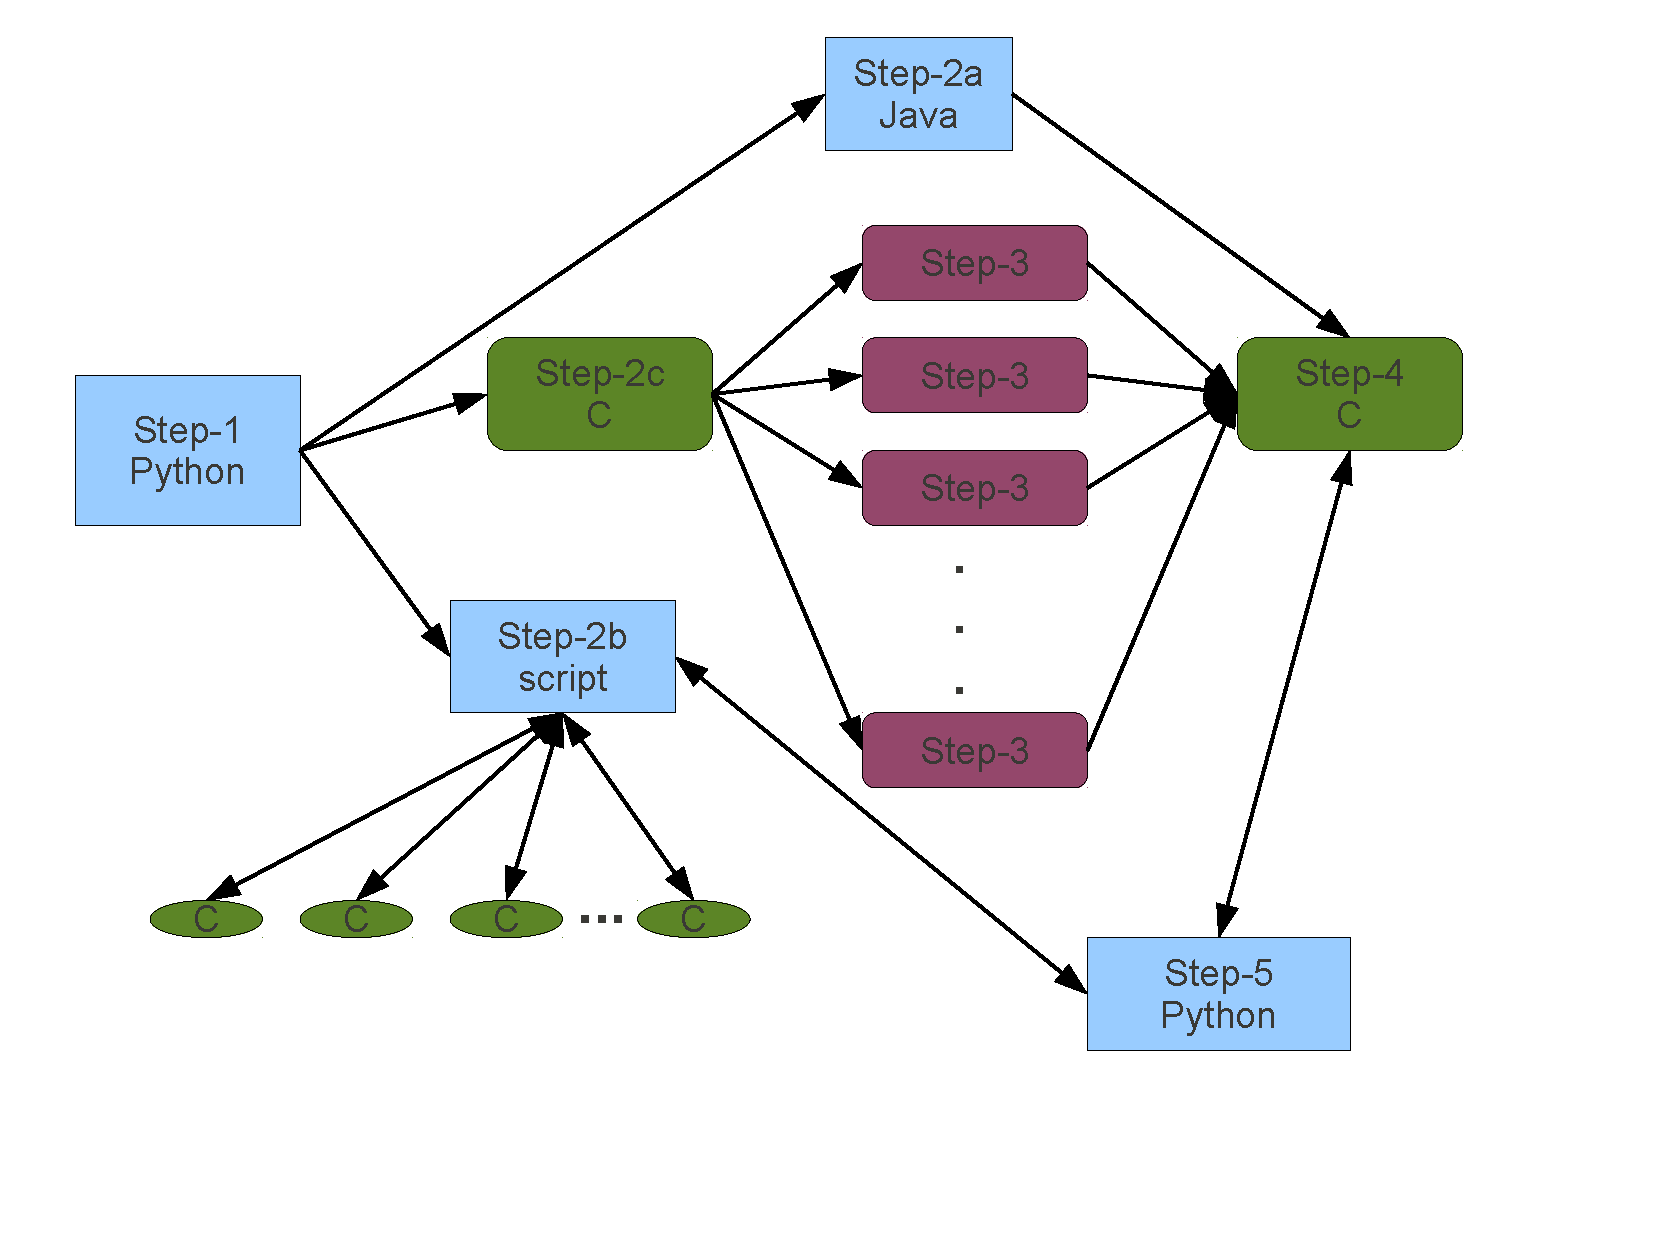
\includegraphics[height=0.3\textheight,width=0.6\textwidth]
		{workFlow}
    \fi
    \caption{Typical dataflow application}	
    \label{fig:dataflow}
  \end{center}
\end{figure}


The increasing popularity of clusters, grids and recent availability of 
cloud computing\cite{ec2} \cite{azure} \cite{appengine} has made the availability of 
these resources commercially feasible for most businesses. But the major obstacle
in widespread adoption is the expertise needed for writing parallel applications.  Also,
dependence on a specific language or runtime environment for parallelism dictates the
need for major re-writing all existing applications for exploiting the parallelism.

Deployment of scientific applications do not focus much on job startup time
as it typically includes deploying a single big application running for a long period.
Most of the performance improvement is measured after the job is started, ignoring
the job startup time.  But dataflow applications typically include running
large number of small applications for short periods of time.  This requirement gives 
significance to job startup time and demands more efficient job deployment solutions.

Another crucial property exhibited by dataflow applications is that the amount of 
resources needed for total computation is unpredictable in the beginning as
it may depend on results of intermediate computations in the DAG.  This leads
to the requirement of dynamically allocating new resources whenever needed.
Most of the current job schedulers do not support such flexibility. 

\subsection{Blue Gene}
Blue Gene \cite{bgp} is a supercomputer aimed at reaching speeds in
the petaFLOPS.  This architecture evolved from Blue Gene/L, Blue Gene/C, Blue Gene/P and Blue Gene/Q.
These are massively parallel machines with 65,536 nodes in the biggest installation.  


Blue Gene is a hierarchical architecture with a controller node at the root managing IO nodes.
Each IO node manages 64 compute nodes, providing distribution and aggregation points for them.
The compute nodes are the leaf nodes responsible for computation.


Compute nodes run a light weight operating system called \textit{Compute Node Kernel(CNK)}.  
CNK is a minimal operating system supporting a subset of the POSIX calls and it allows only one process
to run at a time.  Typically, applications are developed using C, C++ or Fortran with use of 
MPI for communication.  All compute nodes under an IO node are connected with each other using 
the 3D torus network enabling direct point-to-point communication between these compute nodes.


IO nodes run the Linux operating system and are primarily responsible for 
data distribution, aggregation and filesystem operations on behalf of compute nodes.  
It enables compute nodes to communicate with the outside world.
Blue Gene nodes are also connected to each other by the hierarchical tree network 
where IO nodes constitutes a root of a tree of compute nodes.


All IO nodes are connected to a service node which works as a gateway for users
by providing a command interface. The service node runs a Linux operating system and
is mainly responsible for resource reservation using special partitioning.  It
allows multiple users to use Blue Gene by partitioning the nodes into electronically
isolated sets.  This gives isolation and protection to the user applications
which are running simultaneously.  These partitioned nodes are rebooted with a clean 
environment which provides a pristine environment to every user in every reservation.
Once the reservation is over, these partitioned nodes are released.


\subsection{Drawbacks}

Blue Gene was primarily aimed at compute intensive and large scientific applications like 
simulation of protein folding and quantum chemistry.  It is not an ideal environment for 
dataflow applications which mostly consists large
number of small individual applications.  Traditional Blue Gene applications 
are tightly bounded to this environment and do not run anywhere else.  As these
applications don't run on typical workstations, the development and testing process
is difficult and needs access to the Blue Gene setup.  As all applications needs to
be re-developed specifically for this platform, it leads to huge initial investments 
and commitment to this platform which is not desirable for commercial dataflow applications.


In the current setup, every node runs one process, and all nodes in one partition runs the application, 
which makes sense for compute intensive scientific applications.  But typical dataflow applications may not
utilize the entire CPU, leading to in-efficient use of resources.  

The partitioning of nodes is done electronically at the granularity of IO nodes, 
each partition may contain multiple of 8, 16, 32, 64 or 128 nodes.  This base value
is configurable at the hardware level and not at the software level.  So, once any value 
(suppose 64) is chosen, then all partitions on that hardware will contain multiples
of 64 nodes.  As most of the scientific applications are designed to 
scale up or down to any degree of parallelism, absorbing additional nodes available
because of such partitioning is easy.  But typical dataflow applications
are scheduled by treating them as DAG and mapping each computational vertex to a node.
Hence they cannot easily absorb the nodes beyond the number of computational vertices.

Every new reservation leads to the creation of a new partition, and all nodes in that
partition are rebooted.  This leads to a longer job-startup time.  
Again, it does not affect scientific applications much as these applications run for long 
duration.  In contrast, dataflow applications involve starting large number of small jobs.
Many times, these jobs are run multiple times.  Hence
these applications are adversely affected by longer job-startup time.

\subsection{Alternate possibilities}

Recently the Plan 9 \cite{pike95plan} operating system has been ported to the compute
and IO nodes of Blue Gene.\cite{Van07}  Figure 1.2 presents
a new Blue Gene setup with Plan 9.

\begin{figure}[h]
  \begin{center}
    \leavevmode
    \ifpdf
      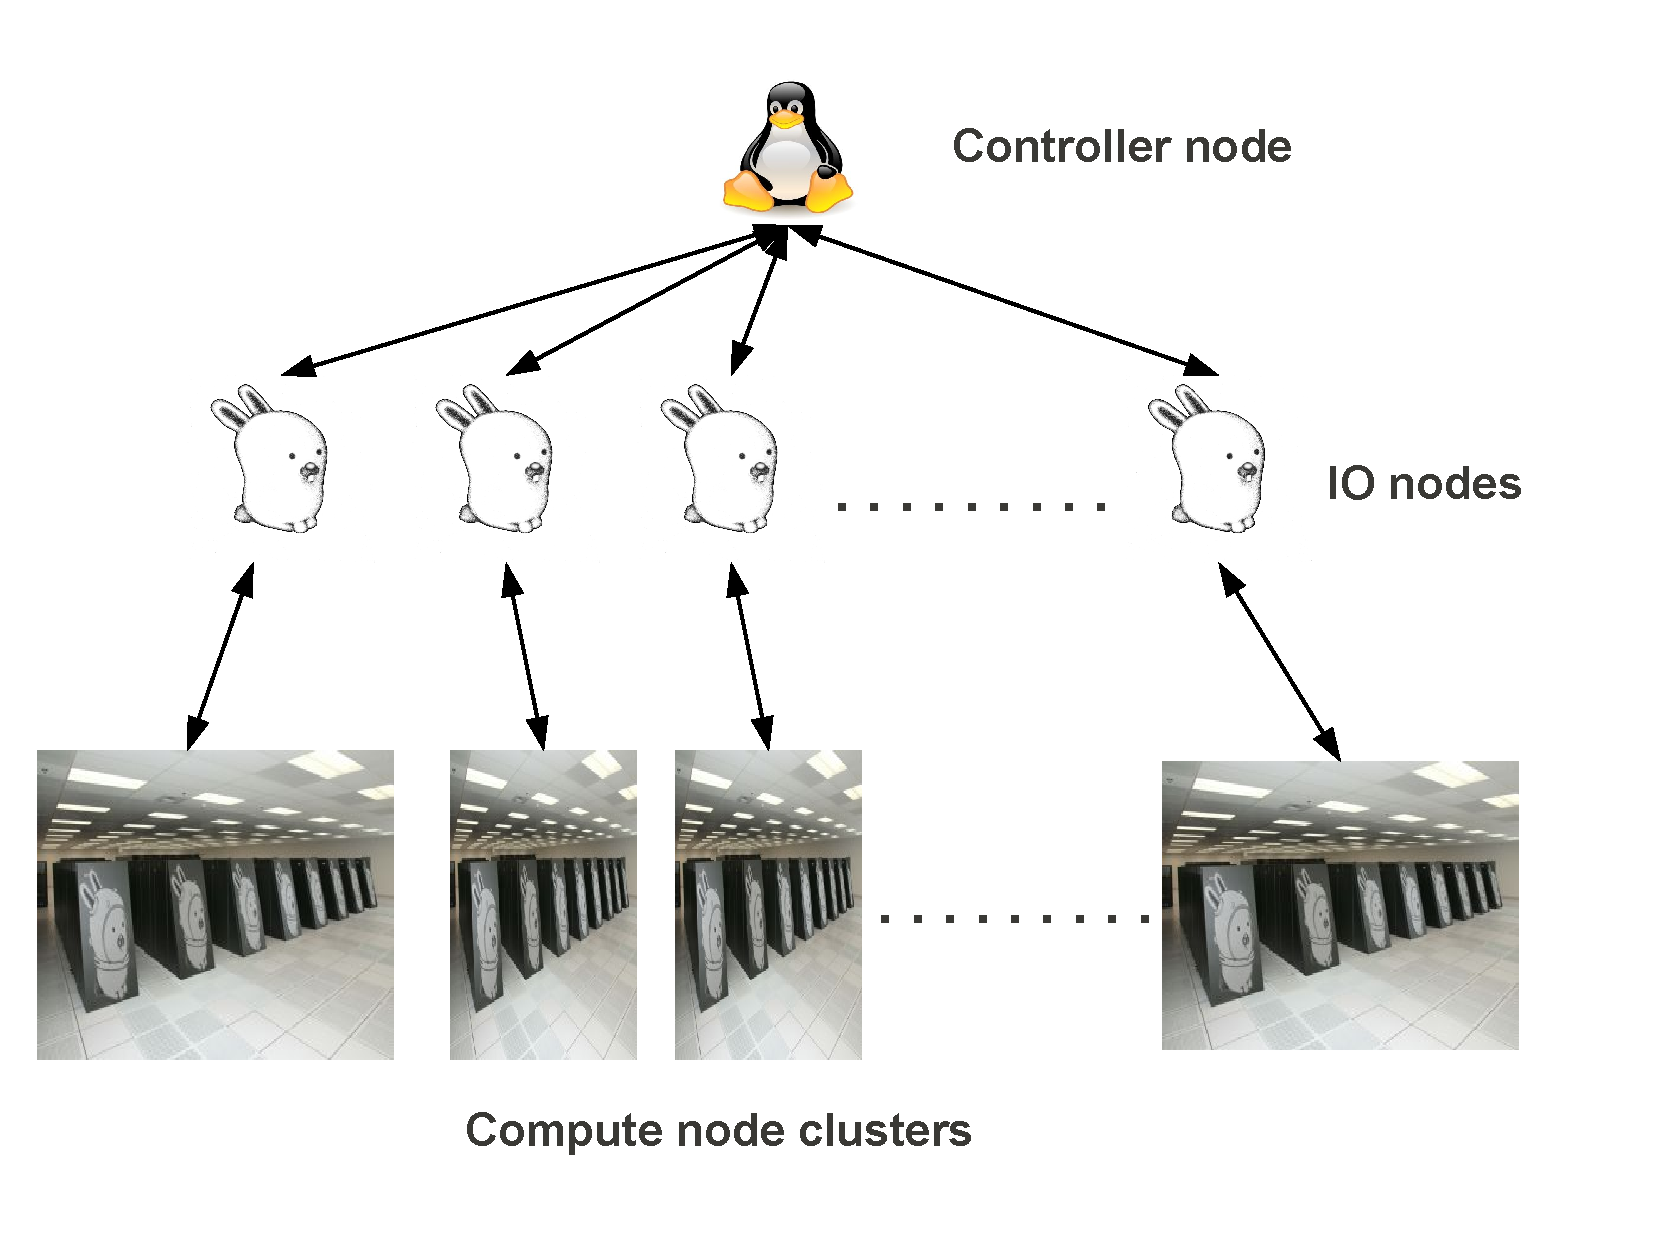
\includegraphics[height=0.4\textheight,width=0.6\textwidth]
		{BlueGeneSetup}
    \fi
    \caption{Bluegene setup}
    \label{fig:bluegene}
  \end{center}
\end{figure}

This setup creates new possibilities for deploying dataflow applications and other
execution models.  With the
availability of Plan 9 on compute nodes we can overcome many limitations posed by
the CNK kernel and availability of Plan 9 on IO node can be used to give much
needed flexibility to dataflow applications.


\section{Goal}
Our goal is to create a scalable infrastructure with the flexibility needed for running dataflow applications.  
We primarily target the Blue Gene supercomputer as our testbed as it allows us to test our infrastructure 
on up to 64K nodes.  Typically, the Blue Gene installations are administered by single
administrative domain.  Also the Blue Gene hardware is designed to provide high reliability.
By relying on these features of Blue Gene, we are able to ignore many complications faced
by typical distributed systems which are aimed to run on unreliable hardware under different administrative domains.
Fault tolerance is a desirable feature of this infrastructure but it is out of scope for this project.

The challenge is to provide the flexibility needed by dataflow applications using a very simple
interface.  We need to provide an infrastructure with support for dynamically adjusting the resource reservation
which can help in coping with unpredictable resource requirements.  This infrastructure
needs to provide quick job-startup time even for large numbers of jobs, allowing overall
good performance for dataflow applications.  It also needs to provide a simple interface
for communication between nodes even when those nodes cannot communicate directly with each other.
We do not want the application development for this infrastructure to be constrained to
a particular language, runtime, middle-ware or platform.  And we need to run most 
of the existing applications without modification.

This project is not aimed at performance improvement, but to present a new and elegant way for
workload distribution and aggregation.  It is aimed at demonstrating that simple filesystem interfaces
and a simple design based on the basic principles of the Plan 9 distributed operating system can be
easy, intuitive and scalable to a large number of nodes.

This project does not aim to entirely solve the problems of dataflow applications, 
but to provide a scalable and flexible infrastructure which can be effectively used to implement them.


This thesis aims to explore alternate possibilities which will simplify the deployment
of dataflow applications on infrastructure like Blue Gene.  Even though we are taking
Blue Gene as a test setup, we aim to develop a generic solution which can be used in any
cluster setup.  The next chapter presents the background work which has inspired this project.  
Chapter 3 will explain the design of our solution.  Chapter 4 will discuss how it is implemented.
Chapter 5 explains the filesystem interface used and shows a few examples to show how easily this
interface can be used.
Chapter 6 presents some evaluations showing that this approach is feasible. Chapter 7 presents
related work and positions this thesis in the context of them.  Chapter 8 will conclude this thesis. 


%%% ----------------------------------------------------------------------

%%% Local Variables: 
%%% mode: latex
%%% TeX-master: "../thesis"
%%% End: 
